\documentclass[12pt,a4paper,twoside]{article}


\usepackage[french]{babel}
\usepackage{fancyhdr}
\usepackage{lastpage}
\usepackage{a4wide} 
\usepackage{amsmath}
\usepackage{amssymb} 
\usepackage{graphicx}
\usepackage{color}
\usepackage{fancybox}
\usepackage{moreverb}
\usepackage{listings}
\frenchbsetup{StandardLists=true}
\usepackage{enumitem}


\title{Charte d'équipe}
\author{Yanis BOUHJOURA, Hugo DABADIE, Garance DUPONT-CIABRINI, Marek ELMAYAN, Julien LALANNE}
\date{\today}


\begin{document}
	\lstset{ numbers=left, tabsize=3, frame=single, numberstyle=\ttfamily, basicstyle=\footnotesize} 
	\thispagestyle{empty}
	
	\begin{center}
		\vspace{1cm}
		
		Grenoble INP  -- ENSIMAG, UGA\\
		École Nationale Supérieure d'Informatique et de Mathématiques Appliquées\\
		\vspace{5cm}
		{\LARGE Projet Génie Logiciel}\\
		\vspace{3cm}
		\shadowbox{
			\begin{minipage}{0.9\textwidth}
				\begin{center}
					{\Huge Charte d'équipe}\\
				\end{center}
			\end{minipage}
		}
	
		\vspace{3cm}
		Yanis BOUHJOURA, Hugo DABADIE, Garance DUPONT-CIABRINI, Marek ELMAYAN, Julien LALANNE \\
		\vspace{3mm}
		GL09 Groupe 2\\
		\vspace{3mm}
		10 janvier 2022\\
		
		
	\end{center}
	

	\newpage
	
	\tableofcontents
	
	\newpage

	\section{Compétences de l'équipe}
		
		\subsection{Fiches d'évaluation}
		
		\vspace{3mm}
		
		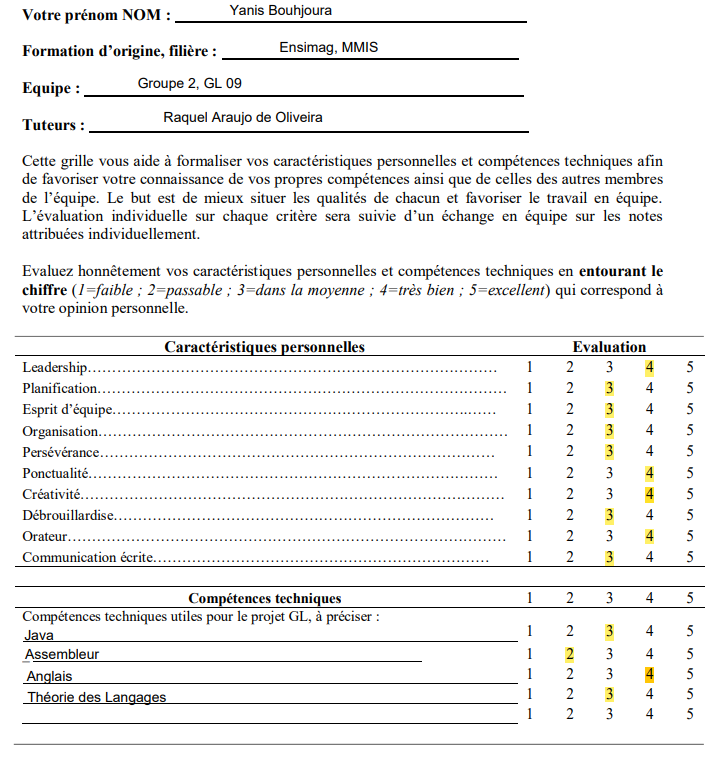
\includegraphics[width=1\textwidth]{Evaluation_Yanis.png}
		\newpage		
		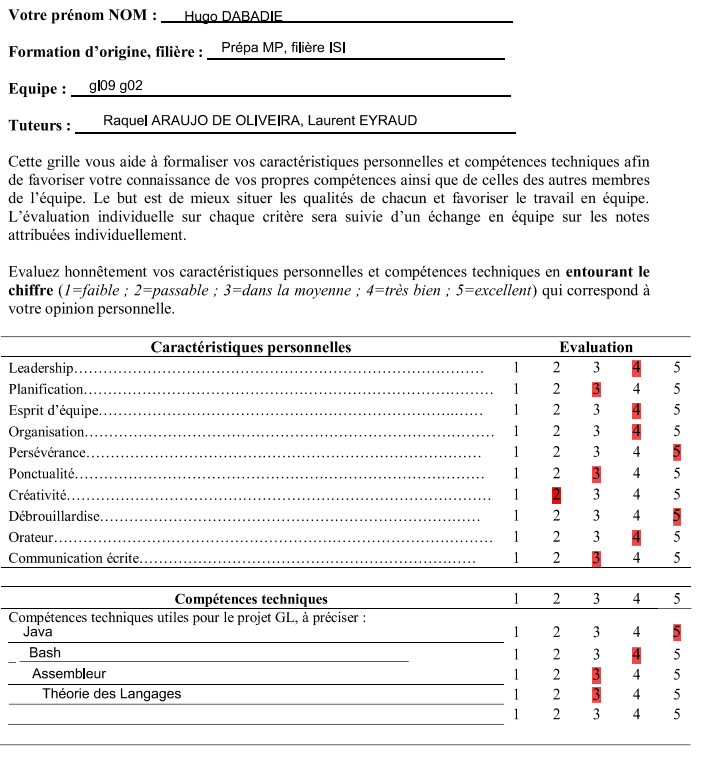
\includegraphics[width=1\textwidth]{Evaluation_Hugo.png}
		\newpage
		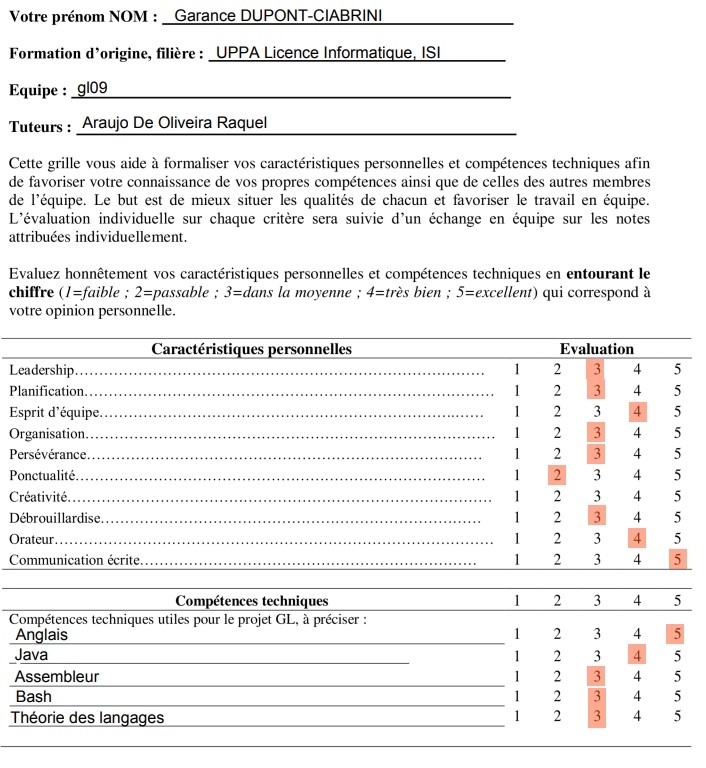
\includegraphics[width=1\textwidth]{Evaluation_Garance.png}
		\newpage
		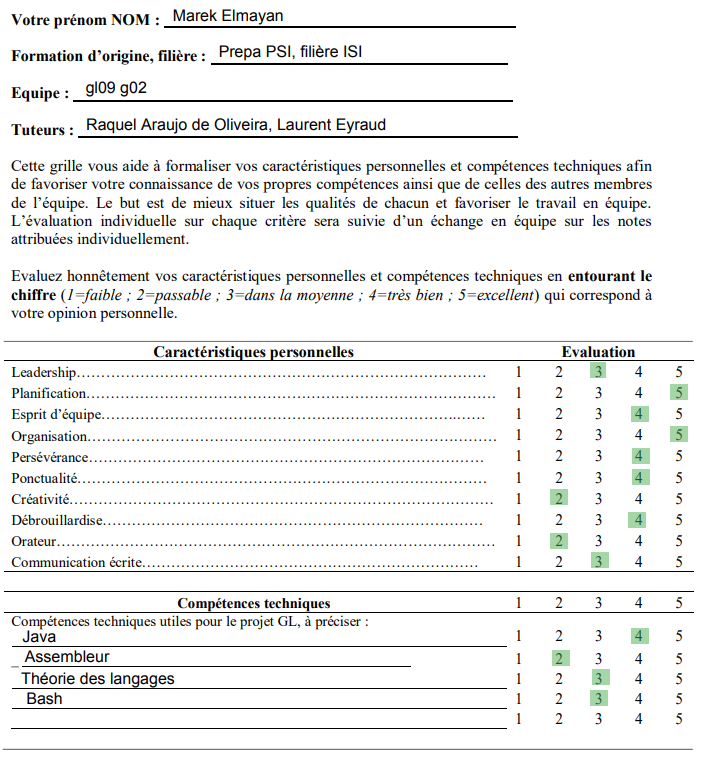
\includegraphics[width=1\textwidth]{Evaluation_Marek.png}
		\newpage
		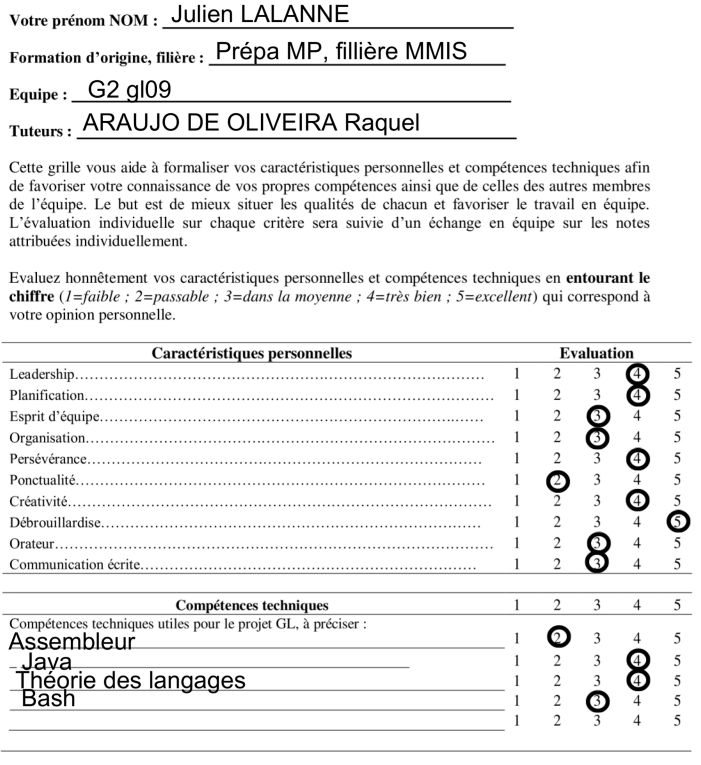
\includegraphics[width=1\textwidth]{Evaluation_Julien.png}
		\newpage
		
		\subsection{Matrice SWOT}
		
		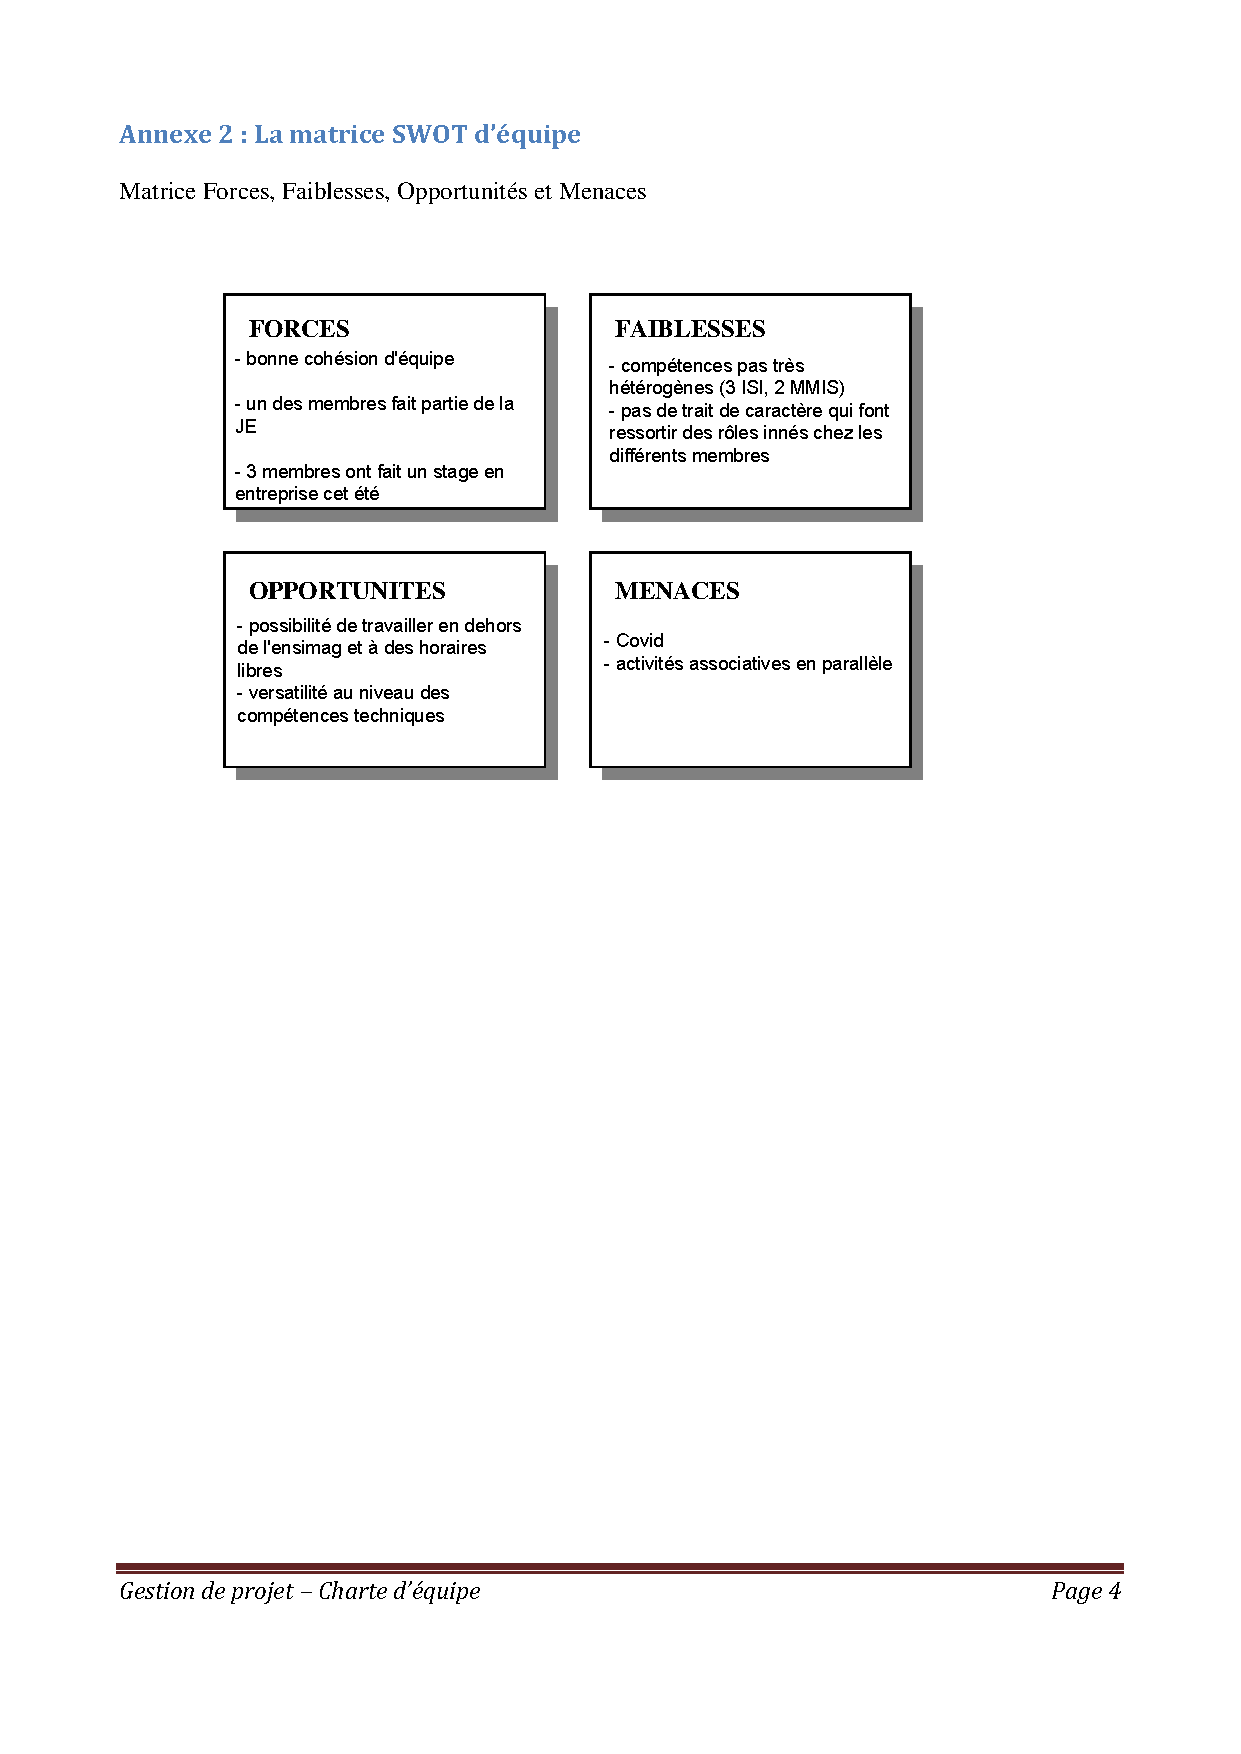
\includegraphics{SWOT.png}
	
	\section{Valeurs communes}
	
	Tout d’abord, notre groupe profite du fait que l’on se connaissait tous avant le début du projet. Ainsi, la confiance entre les membres était assurée dès le départ. Elle n’en reste pas moins une valeur qu’il sera nécessaire de respecter tout au long du projet. Les délais étant courts, il est impossible pour tout le monde d’effectuer des vérifications sur le travail de chacun. Nous avons donc établi cette règle importante : si un des membres du groupe est en difficulté sur sa tâche, il demande rapidement de l’aide et ne cherche pas à masquer ses difficultés; à l’inverse si un membre ne demande pas d’aide, c’est qu’il progresse sur son travail. L’esprit d’équipe associé à la responsabilité personnelle de chacun des membres forment une dualité de valeurs capitale dans la réalisation du projet Génie Logiciel.
	
	$\\$
	
	Dans notre groupe, nous mettons un point d’honneur à nous réunir régulièrement pour mettre en commun l’avancement de chacun (au moins 1 par jour comme le prescrit la méthode Scrum). Cependant, étant donné le nombre de circonstances extérieures (Covid, Activités Associatives importantes…) il nous est impossible d’être 5 à assister à toutes les réunions. De ce fait, la présence à ces dites réunions n’est pas une obligation absolue, néanmoins il est nécessaire qu’un membre absent à une réunion de groupe s’informe sur ce qui a été dit au cours de celle-ci. La bonne diffusion des informations à travers le groupe est clé pour la réussite du projet.
	
	$\\$
	
	Même si notre groupe ne couvre que 2 filières de l’Ensimag, à savoir ISI et MMIS, chacun a une expérience et des connaissances personnelles qui lui sont propres. Ainsi, toute proposition d’un membre mérite d’être écoutée car elle peut se révéler pertinente et apporter une nouvelle vision sur le travail à réaliser.
	
	$\\$
	
	Pour que l’équipe soit la plus performante possible, l’objectif final et les étapes qui permettent d’y arriver doivent être comprises et assimilées par tous les membres. Le planning a donc été mis en place rapidement pour avoir une idée dès le départ des étapes essentielles dans la finalisation du projet. Il est important que tous les membres respectent ce planning et fassent le maximum pour achever leurs tâches dans les délais impartis.
	
	$\\$
	
	Enfin, nous mettons un point d’honneur à reconnaître et mettre en valeur le travail de chacun. Au sein de l’équipe, les réussites individuelles sont célébrées afin que tous les membres ressentent la fierté d’appartenir à l’équipe 09. Un fort sentiment d’appartenance au groupe est crucial pour que chacun s’implique au maximum et sache que son travail sera valorisé. Nous nous permettons notamment des activités de groupe en dehors du projet pour augmenter encore plus la cohésion. Se retrouver dans un autre contexte que celui du projet permet à tout le monde de se reposer et de décompresser tout en partageant des moments avec ses collègues.

	
	\section{Gestion de projet}
	
		\subsection{Méthode utilisée}
		
		Nous avons choisi de nous inspirer grandement de la méthode Agile Scrum afin de faire notre gestion de projet.
		
		$\\$
		
		Nous avons gardé notamment les concepts de Sprints qui correspondront aux grandes étapes du projet. Ses Sprints seront découpés en User Stories qui représenteront les fonctionnalités du projet. Ses User Stories pourront être elles-même découpées en Task représentant une unité de travail.
		
		$\\$
		
		Concernant les artefacts de la méthode Scrum, nous avons choisi d'avoir un Backlog comprenant les différentes User Stories, priorisées, à développer. Tous ces éléments seront présents sur un Task Board que notre outil, ci-après détaillé, permettra de gérer.
		
		$\\$
		
		Pour ce qui est des rituels, nous conservons le Daily Meeting en l'adaptant à notre équipe, dans le sens où nous devrons nous réunir quotidiennement mais pas forcément à horaire fixe. Toutefois, nous ferons un Sprint Planning et un Sprint Review un peu allégé et en même temps, du fait de la taille du projet, dans lesquels nous reviendront rapidement sur le Sprint terminé afin de préparer le prochain.
		
		\subsection{Outils utilisés}
		
		Pour effectuer notre gestion de projet, nous avons choisi d'utiliser Jira. Cet outil est très adapté à la gestion de projet en méthode Agile. En effet, il a été créé pour cela et est très utilisé en entreprise, comme nos stages on permis de nous le montrer.
		
		L'objectif est donc double, avoir un outil puissant à notre disposition pour avoir toutes sortes de fonctionnalités qui permettent de faciliter grandement notre gestion de projet ; mais aussi, apprendre à s'en servir et gagner en expérience. L'apprentissage de l'utilisation de cet outil nous sera bénéfique pour notre vie professionnelle future.
		
		\subsection{Rôles}
		
		Afin d'avoir une organisation permettant de faire le Projet Génie Logiciel dans les meilleures conditions possibles et grâce à l'analyse préalable des compétences de chacun, nous avons décidé de nous répartir les rôles de la manière suivante :
		
		$\\$
		
		\begin{itemize}[label=$\square$]
		
		 \item \textit{Product Owner}, Yanis BOUHJOURA, l'homogéinité de ses caractéristiques personnelles et son bon niveau de créativité notamment sont les raisons qui ont poussé l'équipe à choisir Yanis en tant que Product Owner.
		 
		 Il sera celui qui définira les User Story et qui guidera l'équipe sur les fonctionnalités à développer.
		
		 \item \textit{Scrum Master}, Hugo DABADIE, son expérience en entreprise utilisant la méthode Scrum, avec comme outil Jira, complétée par celle de Junior-Entrepreneur a été l'une des principales raisons du choix de rôle.
		 
		 Il sera le garant du respect de la méthode Agile en veillant à la bonne utilisation des processus Scrum définis.
		
		 \item Development Team :
		 
		 	- \textit{Responsable des tests}, Garance DUPONT-CIABRINI, l'homogénéité de ses compétences techniques nécessaires à la réalisations des tests ainsi que son esprit d'équipe et sa bonne communication permettant de se coordonner avec toute l'équipe, sont les raisons qui ont poussé l'équipe à choisir Garance dans ce rôle.
		 	
		 	Elle sera en charge de définir les tests nécessaires en communiquant à toutes l'équipe et sera le référent sur ce domaine.
		 	
		 	- \textit{Responsable étape C}, Marek ELMAYAN, l'assembleur, au cœur de l'étape C, n'est pas une connaissance que nous avons dans l'équipe. Néanmoins, Marek étant assez débrouillard et à l'aise techniquement, nous avons choisi de le mettre sur cette partie.
		 	
		 	Il devra veiller à la bonne réalisation de cette étape sur l'ensemble du projet et sera là pour conseiller les autres membres de l'équipe.
		 	
		 	- \textit{Responsable étape A et B}, Julien LALANNE, étant la personne la plus à l'aise avec la théorie du langage, au cours de ces deux étapes, Julien a été choisi pour ce rôle.
		 	
		 	Il devra veiller à la bonne réalisation de ces deux étapes sur l'ensemble du projet et sera là pour conseiller les autres membres de l'équipe.
		 	
		 \end{itemize}
		 	
		$\\$
		 	
		 Les rôles sont là pour avoir un référent dans chaque tâche à faire mais chaque membre de l'équipe a la possibilité d'aider n'importe quel membre dans son domaine. Les responsables sont là pour assurer que le projet soit mené au bout de son terme mais ils ne sont en aucun cas les seuls à travailler sur leur partie du projet.
		 
		 De plus, les rôles ne sont pas fixes et pourront évolués au fil du projet si cela est nécessaire dans l'intérêt de la réalisation du projet.
		
		
	\section{Communication au sein de l'équipe}
		
		\subsection{Organisation de la communication}
		
		La communication commence d'abord par le respect des rituels définis plus haut qui permettront d'assurer une communication régulière et efficace au sein de l'équipe, notamment grâce aux Daily Meetings.
		
		L'objectif est d'essayer de faire ces derniers un maximum en présentiel, à l'Ensimag ou chez un des membres de l'équipe. Si cela n'est pas possible, on maintiendra tout de même ces rituels à distance grâce à l'utilisation d'outils adaptés.
		
		La communication dans notre équipe s'organise aussi naturellement du fait que Garance et Julien habitent ensemble, Yanis habite très proche d'eux et Marek et Hugo habitent également ensemble.
		
		\subsection{Outils}
		
		Les outils de développement que nous utilisons sont un IDE (VSCode et IntelliJ), permettant d'avoir un développement facilité et Gitlab, permettant un historique des versions qui servira éventuellement en cas d'erreur à revenir en arrière mais surtout qui a pour objectif un échange facile des fichiers du projet.
		
		Pour communiquer, les outils utilisés sont une conversation Messenger, pour la spontanéité et la rapidité des réponses, Discord, pour une organisation des messages plus efficace et Jira, dans une autre mesure, pour notamment discuter sur un point spécifique du projet lors du développement. Aussi, Discord permet une communication à distance efficace grâce au partage d'écran notamment.
		
		\subsection{Réunions}
		
		Nous organisons des réunions comme défini ci-dessus dans notre adaptation des processus Scrum dans le but de maintenir une communication efficace et que chaque personne de l'équipe est une idée globale de l'avancée du projet.
		
		$\\$
		
		Les Daily Meetings nous permettent chaque jour de revenir sur les difficultés rencontrés afin de les résoudre et d'exposer le travail qui va être effectué dans la journée à venir.
		
		$\\$
		
		Les réunions de fins de Sprint, elles, sont là afin de prendre les points négatifs et positifs du Sprint qui vient de se terminer pour garder ce qui allait et changer ce qui n'allait pas.
		
		$\\$
		
		Il est également possible à tout moment, par n'importe quelle personne, de demander une réunion exceptionnelle qui permettra de résoudre une situation de crise.
		
		$\\$
		
		Le Scrum Master est chargé d'aminer ses différentes réunions. Il n'y aura pas nécessairement de compte-rendu pour les Daily Meetings, sauf en cas d'absence d'un des membres de l'équipe. Cependant, il est fortement recommandé de rédiger un compte-rendu synthétique des réunions de fin de Sprint.
		
		La personne en charge de rédiger un compte-rendu est désigné par l'ensemble de l'équipe au début de la réunion.
		
		\subsection{Gestion des difficultés}
		
		Même si nous faisons notre maximum pour que le groupe reste soudé, il est irréaliste de penser qu’aucune tension ne pourrait apparaître au sein de l’équipe. Nous avons donc dû réfléchir au préalable à des moyens de les éviter ou dans le pire des cas de les gérer. Nous pensons que la communication est la clé pour éviter tout conflit au sein d’un groupe. Les réunions récurrentes et les activités extra-professionnelles que nous avons mis en place ont pour objectif de permettre cette communication et de confronter les problèmes au lieu de les laisser grandir et devenir des sources de tensions.
	
	
\end{document}
